\documentclass[aspectratio=169]{laplace-beamer}

%\input{preamble}

%\setbeameroption{show notes on second screen}
%\draft
% \webcast
%\setbeamercolor{alerted text}{fg=supelecRed!20!red!80}
% \usetikzlibrary{overlay-beamer-styles}
%\bibliography{../../../bibliography.bib}

%\title[Short Version of the Title]
%{This is my very very very very\\ long title}
\title[Short Version of the Title]
{This is my Title}

% \subtitle
% {And this is the subtitle}

\author[Author SURNAME] % (optional, use only with lots of authors)
{Author SURNAME\\
\texttt{author.surname@email.com}}

\date{25/05/2023}
\subject{}

% Delete this, if you do not want the table of contents to pop up at
% the beginning of each subsection:
\AtBeginSection[]
{
  \begin{frame}<beamer>[alternate_watermark]{Outline}
    \tableofcontents[sectionstyle=show/hide,subsectionstyle=show/show/hide]
  \end{frame}
}

\begin{document}

\begin{frame}[plain]
  \titlepage[banque/Image16.png]%
\end{frame}

\begin{frame}{Sommaire}
  \tableofcontents[subsectionstyle=hide/hide/hide]
\end{frame}

\section{Model of pages}
\subsection{Default}
\begin{frame}{This my horrendous, really big (enormous) title}{And this is also a subtitle}
    \lipsum[1][6]
\end{frame}

\subsection{Alternate Watermarks}
\begin{frame}[vertical_watermark]{This my horrendous, really big (enormous) title}{Vertical watermark is better for long tittles}
    \lipsum[1][5]
\end{frame}

\begin{frame}[alternate_watermark]{Alternate Watermark}{This is yet another watermark}
    \lipsum[1][2]
\end{frame}

\begin{frame}[default]{Default page}{Going back to default}
    \lipsum[1][1]
\end{frame}

\begin{frame}{Default page}{Do not need to mention \texttt{[default]} framekey again}
    \lipsum[1][1]
\end{frame}

\subsection{Big with an image}
\begin{frame}[big_image_right={banque/Image20.jpg}]{Text + image portrait}{Here we use a minipage to contain text}
  \begin{minipage}{.45\textwidth}
    \begin{block}{Lorem Ipsum}
      \lipsum[1][1-6]
    \end{block}
  \end{minipage}
\end{frame}

\section{Some Examples}
\begin{frame}[default]{Penultimate Slide}
\end{frame}

\begin{frame}{One Image}
\begin{figure}[ht]
  \centering
  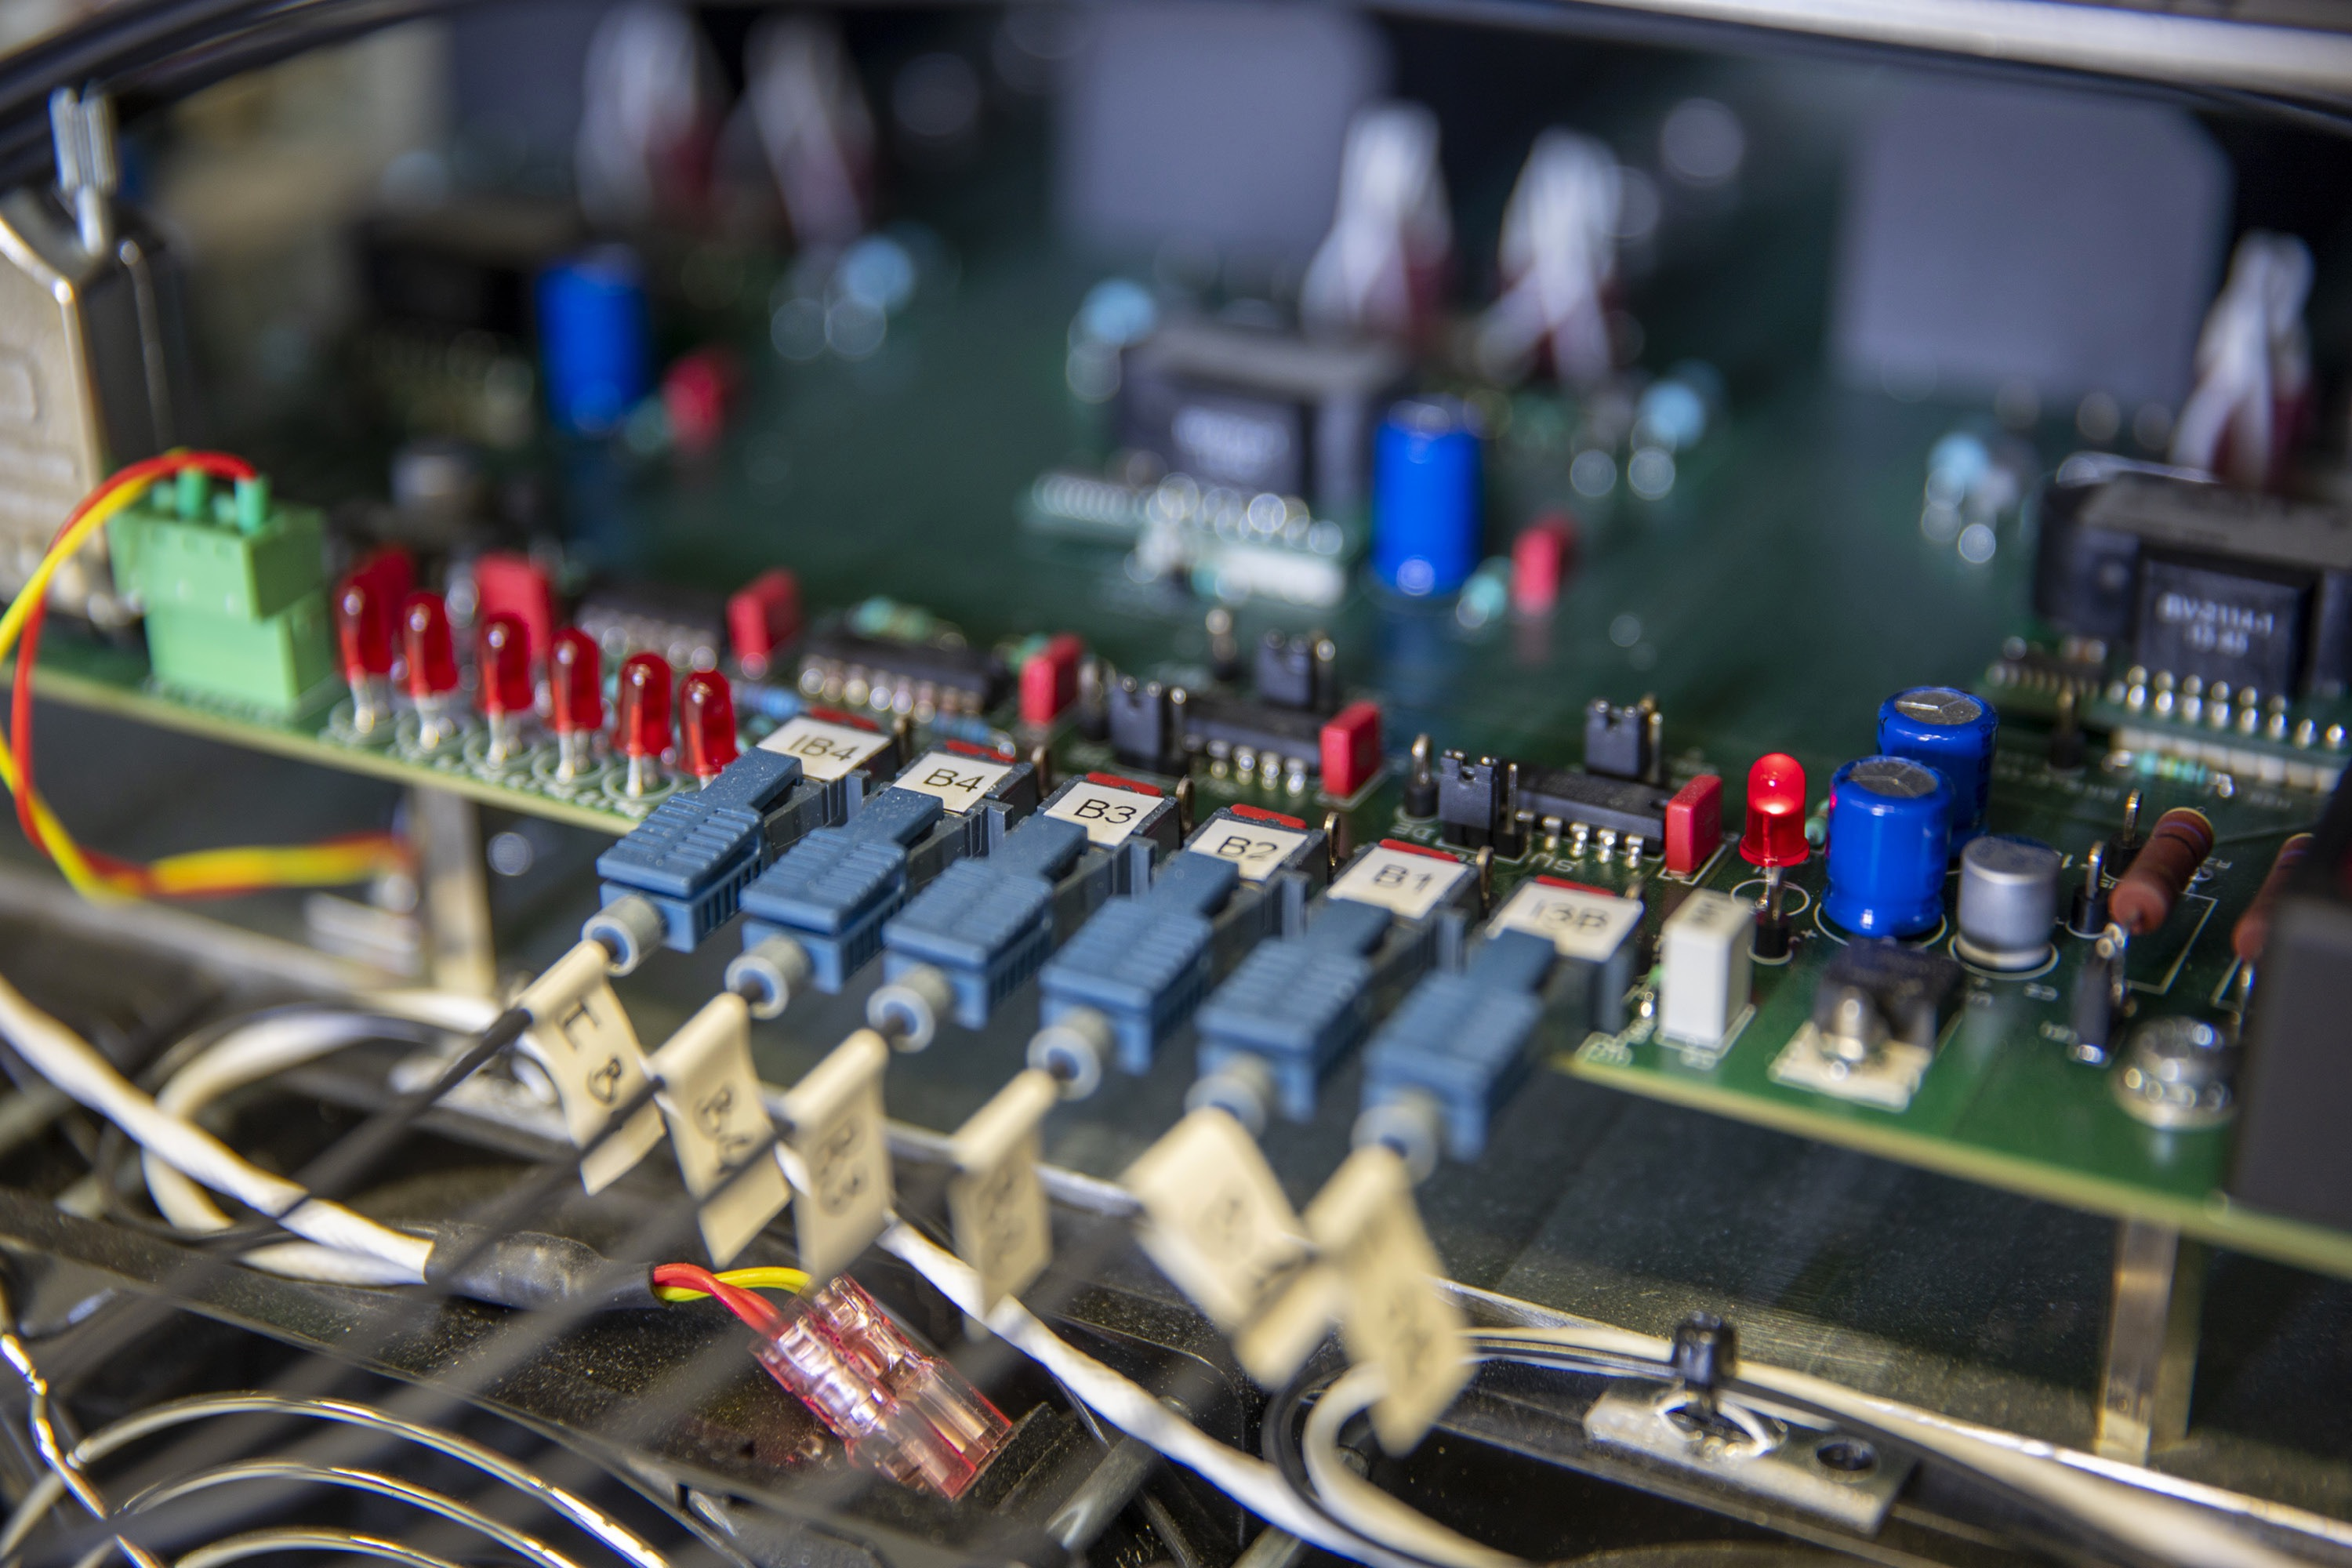
\includegraphics[width=0.5\textwidth]{banque/Image20.jpg}
  \caption{My cool figure}
\end{figure}
\end{frame}

\begin{frame}{Image and Text side-by-side}
  \begin{minipage}[c]{0.45\textwidth}
    \begin{figure}[ht]
      \centering
      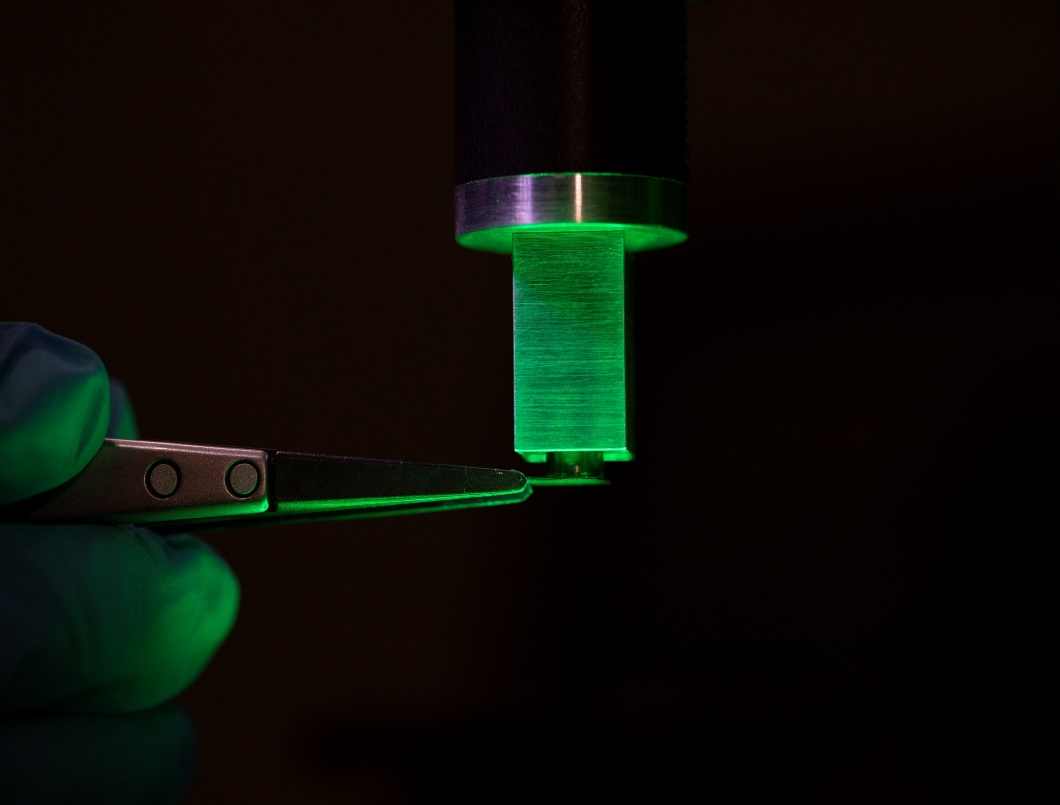
\includegraphics[width=1\textwidth]{banque/Image22.jpg}
      \caption{My other cool figure}
    \end{figure}
  \end{minipage}
  \hfill
  \begin{minipage}[c]{0.45\textwidth}
    \begin{block}{Lorem Ipsum}
      \lipsum[1][1-6]
    \end{block}
  \end{minipage}
\end{frame}

\begin{frame}{Image and Enumerate side-by-side}
  \begin{minipage}[c]{0.45\textwidth}
    \begin{figure}[ht]
      \centering
      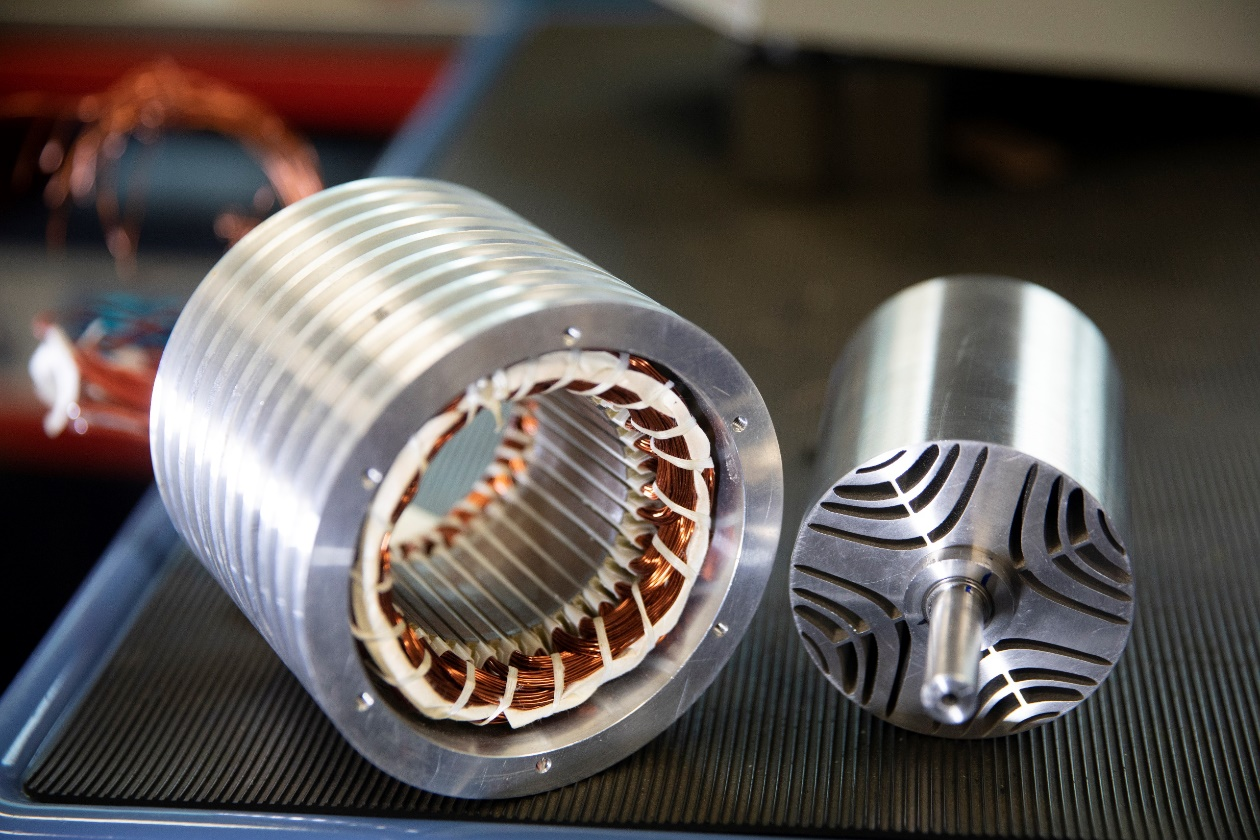
\includegraphics[width=1\textwidth]{banque/Image23.jpg}
      \caption{Wow another cool figure}
    \end{figure}
  \end{minipage}
  \hfill
  \begin{minipage}[c]{0.45\textwidth}
    \begin{block}{Lorem Ipsum}
      \begin{enumerate}
        \item Item
        \item Item
              \begin{itemize}
                \item Item
                \item Item
                \item Item
              \end{itemize}
        \item Item
      \end{enumerate}
    \end{block}
  \end{minipage}
\end{frame}

\begin{frame}{Equation and Enumerate side-by-side}{Here we alert that $c$ is important}
  \begin{minipage}[c]{0.45\textwidth}
    \begin{equation*}
      \label{eq:1}
      E=m\alert<2>{\tikzmarktext{speed1}{$c$}}^{2}
    \end{equation*}
  \end{minipage}
  \hfill
  \begin{minipage}[c]{0.45\textwidth}
    \centering
    \begin{block}{My equation}
      \begin{itemize}
        \item[$E$] Energy
              \begin{itemize}
                \item[$m$] Mass
                \item[$\tikzmarktext{speed2}{c}$] Speed of light
              \end{itemize}
      \end{itemize}
    \end{block}
  \end{minipage}
  \begin{tikzpicture}[overlay, remember picture]
    \alert<3>{\draw<3-4> (speed1.south) edge[thick,out=-90,in=180,->] (speed2.west);}
  \end{tikzpicture}
\end{frame}

\begin{frame}[plain]
  \endpage%
  \centering
  Thank you
\\~\\
  Questions? Comments?
  \\~\\
  \insertauthor
\end{frame}


\end{document}

%%% Local Variables:
%%% mode: latex
%%% TeX-master: t
%%% End:
